\chapter{Literature Review}
\label{chap:literature_review}

The \gls{VRP} and the \gls{CVRP} belong to the most frequently studied combinatorial
optimization problems, and are proven $NP$-hard. The goal is to minimize the total driven distance
by a fleet of vehicles, which have to start and end each tour at a central depot driving to each
customer exactly once.\footcite[cf.][p. 1]{gendreau_tabu_2008} Some \gls{VRP}
instances constructed from \cite{solomon_algorithms_1987} could not be solved optimally until now and the
solvation leaded rallys to solve them.\footcite[cf.][]{solomon_algorithms_1987} However,
in practical and real-world situations items can not be considered as integers of weight
and volume to check the loading, but by considering the geometrical shape and characteristics.\footcite[cf.][p. 1]{gendreau_tabu_2008}
To attain a more realistic profile of routing and loading problems, \cite{iori_exact_2004} and \cite{gendreau_tabu_2008}
solved the \gls{2L-CVRP} for the first time, considering the area of each item in
the delivery vehicles.\footcites(cf.)(){iori_exact_2004}{gendreau_tabu_2008}
This lead consequently to a more complex problem, as every route needed to be checked separately for
a feasible loading without violating physical and loading related constraints.
The applicability in practical scenarios was further increased from \cite{gendreau_tabu_2006} by defining
the \gls{3L-CVRP}, considering the stacking of items and three-dimensional items and vehicles. The authors
also conidered a set of practical loading constraints to further enhance the applicability. \footcite[cf.][]{gendreau_tabu_2006}
The algorithms to solve the integrated problems could already be taken from existing literature tackling the standalone
problems, \gls{CLP} and \gls{VRP}.\footcite[cf.][]{pisinger_heuristics_2002} Foremost, the following section defines
a mathematical model formulation for the \gls{3L-CVRP} and the following literature review will focus
on the \gls{CLP}, its possible constraints, algorithms to solve it and the possibility to use solution
methods beside the classical approaches. As the \gls{CLP} is considered as a subproblem of the \gls{VRP}
in this thesis, the literature and examples refer to the \gls{3L-CVRP} and each problem should not be
considered solely.

\section{Mathematical formulation}
\label{sec:mathematical_formulation}

This two-index vehicle flow formulation for the \gls{3L-CVRP} is taken from \cite{tamke_branch-and-cut_2024}.\footcite[cf.][pp. 6-7]{tamke_branch-and-cut_2024}
The advantage is that infeasible tours of the subproblem \gls{CLP} are excluded
as route candidates for the masterproblem \gls{VRP} and no loading constraints are directly defined in the model, but in the rules
to exclude routes from the solution process. First, the used sets and prameters are presented and afterwards the constraints with
explainations.

\subsection*{Sets}
A directed graph $G=(N,A)$ is defined by the set of nodes $N$ including the depot and the set of arcs
$A = \{ (i, j) \mid i, j \in N \}$ between all nodes. The set of customer nodes $C$ is defined without the depot.
The Sets $\delta^+$ and $\delta^-$ define the arcs, which are leaving respective entering a node.
For example, for node 3, $\delta^+ = \{(3,5)\}$ and $\delta^-= \{(2,3)\}$.
The set $A(S)$ defines a sequence of arcs connecting nodes in a random set of customers $C$,
which is a route in wider sense. For example the set $A(S)=\{(2,1),(1,5),(5,3)\}$ connects nodes
2 and 3 via node 5. Every set $A(S)$ is defined by the total volume $q(S)$ and total weight $v(S)$
demanded by all customers $i \in S$, with $S \subseteq C$. The set $A(P)$ includes all infeasible sequences $P$ leading
to an infeasible route.

\begin{table}[ht]
    \centering
    \begin{tabular}{llc}
        \toprule
        Symbol        & Description                              & Range                         \\
        \midrule
        $N$           & Set of nodes                             & $\{ 0, \dots, N \}$           \\
        $C$           & Set of customers                         & $\{ 1, \dots, N \} $          \\
        $A$           & Set of directed arcs                     & $\{(0,1), \dots, (n-1, n) \}$ \\
        $\delta^+(i)$ & Set of arcs leaving node $i$             & $\in A$                       \\
        $\delta^-(i)$ & Set of arcs entering node $i$            & $\in A$                       \\
        $A(S)$        & Set of arcs with both ends in subset $S$ & $\in A$                       \\
        $A(P)$        & Set of arcs in an infeasible path $P$    & $\in A$                       \\
        \bottomrule
    \end{tabular}
\end{table}
\vspace{0.2em}

\subsection*{Parameters}
The parameters can be divided in the two groups, static and set-dependent
The costs $c_{ij}$ for travelling from one node $i$ to another node $j$,
are symmetrical defined, stating $c_{ij} \overset{!}{=} c_{ji}$. Furthermore, the triangle inequality
$c_{ij} \leq c_{ih} + c_{hj}$ needs to be fulfilled, that the travel distance is always shorter travelling
directly and not via any intermediate node $h$. Additionally the number of vehicles
available for the fleet planning is given as constant $K$. No solution is allowed to have
more routes than avalaible vehicles. $r(S)$ defines a \gls{LB} for the numbers of vehicles needed
to include all customers in $S$. The \gls{LB} is calculated as the ceiling of the maximum
value between the total weight $q(S)$ divided by the weight capacity $Q$, and the
total volume $v(S)$ divided by the volume capacity $V$:
\[r(S) = \max\left( \left\lceil \frac{q(S)}{Q} \right\rceil, \left\lceil \frac{v(S)}{V} \right\rceil \right)\]

\begin{table}[ht]
    \centering
    \begin{tabular}{ll}
        \toprule
        Symbol   & Description                                                   \\
        \midrule
        $c_{ij}$ & Cost or distance of traveling from node $i$ to node $j$       \\
        $K$      & Number of available vehicles                                  \\
        $Q$      & Weight limit of vehicle                                       \\
        $V$      & Volume limit of vehicle                                       \\
        $q(S)$   & Total weight requested by customers in $S$                    \\
        $v(S)$   & Total volume requested by customers in $S$                    \\
        $r(S)$   & Minimum number of vehicles required to cover customers in $S$ \\
        \bottomrule
    \end{tabular}
\end{table}

\bigskip

\subsection*{Decision Variable}
For the Two-Index-Flow model only one binary decision variable is necessary stating, if the arc
between nodes $i$ and $j$ is included in the solution.
\[
    x_{ij} =
    \begin{cases}
        1 & \text{if arc } (i,j) \text{ is used in the solution} \\
        0 & \text{otherwise}
    \end{cases}
\]

\bigskip

\subsection*{Model}
\textbf{Objective:}
\begin{equation}
    \label{eq:objective}
    \min \sum_{(i,j)\in A} c_{ij}x_{ij}
\end{equation}

\textbf{Subject to:}
\begin{align}
    \sum_{(i,j)\in \delta^+(i)} x_{ij} & = 1                                                                                  &  & \forall i \in C                         \label{eq:flowout}     \\
    \sum_{(i,j)\in \delta^-(i)} x_{ij} & = 1                                                                                  &  & \forall i \in C                         \label{eq:flowin}      \\
    \sum_{(i,j)\in \delta^+(0)} x_{ij} & \leq K                                                       \label{eq:vehiclelimit}                                                                     \\
    \sum_{(i,j)\in A(S)} x_{ij}        & \leq |S| - r(S)                                                                      &  & \forall S \subseteq C, S \neq \emptyset \label{eq:capacitycut} \\
    \sum_{(i,j)\in A(P)} x_{ij}        & \leq |A(P)| - 1                                                                      &  & \forall \text{ infeasible paths } P     \label{eq:pathelim}
\end{align}

The objective function minimizes the total costs and the travelled distance. The constraints \ref{eq:flowin}
and \ref{eq:flowout} are restricting that every customer can and must only be visited once by defining the number
of arcs leaving and entering a node $i$ to 1. These two constraints do not apply to the depot,
which is included in every tour. Constraint~\ref{eq:vehiclelimit} limits the maximum number of
tours to $K$ by limiting the number of arcs entering the depot ($(i,j)\in \delta^+(0)$).
The next constraint~\ref{eq:capacitycut} states, that the number of arcs within the subset $A(S)$
must be smaller or equal to the number of customers minus the \gls{LB} for vehicles. This constraint
ensures, that routes are connected to the depot and that each subset $S$ is not violating
the volume and weight capacities. For example, if $S=\{1,2,3\}$ with $A(S)=\{(2,3),(3,1)\}$
and $r(S) = 1$, then $2 \leq 3 - 1$ holds, but if the \gls{LB} would be instead 2 then, $2 \not\leq 3 - 2$
and two tours need to be constructed. The last constraint~\ref{eq:pathelim} excludes all infeasible paths
$P$ from the solution. Every path $P$ is defined by a subset of arcs $A(P)$ defining it. Infeasible
paths are labeled as such, when the corresponding \gls{CLP} to a route is not fulfilling the loading
constraints. The constraint determines, that at least one binary variable defining an arc
from the set of arcs defining the infeasible path $|A(P)|$ has to have the value 0, that the left
side of this constraint is smaller equal to the right side. The set of infeasible paths is determined by
solving the subproblem of the \gls{CLP}.






\section{Container Loading Problem}
\label{sec:clp_definition}

The placement and assignment of items to larger, mostly rectangular
containers, is a well known problem in logistics and operations research, as the
potential of cost savings and efficiency gains is substantial by reducing the number
of needed containers or by fulfilling customer needs. The \gls{CLP} covers a broad range of real-world applications,
such as loading cargo, optimizing warehouse storage and packing of pallets or cardboard boxes.
Generally, it is differentiated in \textit{input minimization},
where the number of needed containers is minimized, and \textit{output maximization} problems,
where the value of the associated items is maximized. The \gls{BPP} is the generalized problem type of the \gls{CLP}
and belongs to \textit{input minimization} problems, whereas the knapsack problem to \textit{output maximization}.
Apart from the expected outcome of the optimization,
the characterics of the items and containers is crucial for the problem definition. Items can be either
homogeneous or heterogeneous in size and shape. Furthermore, they can be classified as weakly or strongly
homogeneous or heterogeneous, depending on the degree of similarity among them. The container is
defined as a rectangular volume with a fixed size and shape, where the items have to be placed in.
Other, non rectangular, shapes are seldomly considered in the literature, as the practical relevance is
limited.
Multiple containers of homogeneous or heterogeneous sizes are used when the volume and weight
of the cargo require it.
According to \textcite{bischoff_issues_1995}, the mere placement of items in containers is insufficient
if practical requirements are not fulfilled as it lacks applicability.
\textcite{bortfeldt_constraints_2013} systematically categorized all constraints emphasized in \gls{CLP} research
into five categories, which are presented in the following. They also distinguish between hard and soft constraints,
where hard constraints must be strictly satisfied, while soft constraints may be violated
to some extent.\footcites(cf.)()[p. 1f]{bortfeldt_constraints_2013}[p. 1f]{bischoff_issues_1995}

\subsubsection{Container related constraints}
These constraints summarize all physical barriers of the container. The \textit{load capacity} limits the aggregated
mass of all items in the container. The distribution of the weight (\textit{load balance})
plays an important role for safety reasons, as the cargo must not move during the transport and the container
must not tip over. It is defined by the maximum weight difference between the left and right half of the container.
When the containers are transported by trucks, uneven \textit{axle weight} distribution can cause severe
consequences and needs to be avoided for practicability by loading the cargo axle-friendly. \footcite[cf.][p. 849f]{krebs_advanced_2021}

\subsubsection{Item related constraints}
Item related constraints define the properties of the item, which are relevant
for the packing. When the container capacity is limited (\textit{output maximization}),
the \textit{loading priority} constraint defines the priority among possible
item candidates. The \textit{orientation} constraint restricts how an item can be rotated.
There are several types of rotation, each defined by the axis around which the item rotates.
The most common is the \textit{z-rotation}, where rotation is only allowed around the vertical axis.
When 3D packing is considered, stacking of items is allowed in comparison to 2D packing, when all
items are placed on the container floor. Two main approaches exist, when stacking is considered.
The \textit{fragility} constraint differentiates between fragile and non-fragile items,
allowing only non-fragile items to be stacked on non-fragile items. Figure \ref{fig:stacking_comparison} showcases
this definition. The other approach defines an individual \textit{\gls{LBS}} for each
item stating how much pressure the box can tolerate, and which items can be stacked. \footcite[cf.][p. 847f]{krebs_advanced_2021}

\begin{figure}[htbp]
    \centering
    \small
    % First TikZ picture
    \begin{subfigure}[b]{0.45\textwidth}
        \centering
        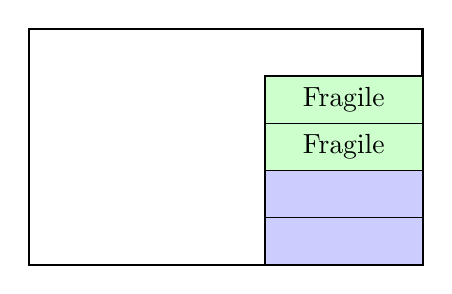
\begin{tikzpicture}
            % Draw the container
            \draw[thick] (0,0) rectangle (5,3);

            % Draw the three items inside
            \draw[fill=blue!20] (3,0) rectangle (5,0.6);
            \node at (4, 0.3) {};

            \draw[fill=blue!20] (3,0.6) rectangle (5,1.2);
            \node at (4, 0.9) {};

            \draw[fill=green!20] (3,1.2) rectangle (5, 1.8);
            \node at (4, 1.5) {Fragile};

            \draw[fill=green!20] (3,1.8) rectangle (5, 2.4);
            \node at (4, 2.1) {Fragile};

        \end{tikzpicture}
        \caption{Feasible stacking of items.}
    \end{subfigure}
    \hfill
    % Second TikZ picture
    \begin{subfigure}[b]{0.45\textwidth}
        \centering
        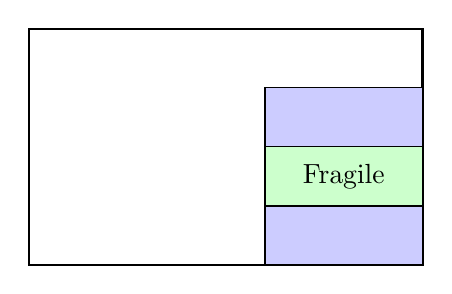
\begin{tikzpicture}
            \draw[thick] (0,0) rectangle (5,3);

            % Draw the three items inside
            \draw[fill=blue!20] (3,0) rectangle (5,0.75);
            \node at (4, 0.5) {};

            \draw[fill=green!20] (3,0.75) rectangle (5,1.5);
            \node at (4, 1.125) {Fragile};

            \draw[fill=blue!20] (3,1.5) rectangle (5, 2.25);
            \node at (4, 1.875) {};
        \end{tikzpicture}
        \caption{Infeasible stacking of items.}
    \end{subfigure}
    \caption[Visualization of fragility constraint.]{Comparison of fragile stacking (side view).}
    \label{fig:stacking_comparison}
\end{figure}


\subsubsection{Cargo-Related Constraints}
In contrast to item-related constraints, cargo-related constraints apply to
the entire cargo or to specific subsets of it. The \textit{complete-shipment} constraint
requires that all items within a shipment must either be loaded into the same
container or be left behind entirely. This constraint is important
when container capacity is limited (\textit{output maximization}) and items
cannot be split. The \textit{allocation} constraint serves a similar purpose,
including the \textit{connectivity} constraint, which mandates that
certain items must be loaded into the same container, and the
\textit{separation} constraint, which requires specific items to
be distributed across different containers. For example, kitchen
shipments, comprising multiple packages, should be delivered together
to enable efficient installation. Conversely, items such as perfume and fresh
vegetables should be shipped separately due to incompatibility.

\subsubsection{Positioning constraints}

Positioning constraints determine, if items must be placed at
absolute locations or relative to other items. Absolute positioning is
typically based on item characteristics such as size, weight, or
content (e.g., bulky or hazardous items placed near the container door for accessibility) or
they may universally apply to all items, as the \textit{geometry} and
\textit{orthogonality} constraints. These constraints define that items are not allowed to overlap
and must be placed orthogonally to the container walls respectively.
Relative positioning requires items to be placed either close together as a \textit{group} or
\textit{separated} from each other.
The multi-drop constraint combines absolute and relative positioning requirements for items
destined for different delivery locations. The goal is to minimize reloading efforts by grouping items
by destination, arranging these groups in the delivery sequence, and applying either a \textit{\gls{LIFO}}
or sequential loading policy to ensure efficient unloading without having to move unrelated items.
Variations of the \gls{LIFO} constraint account for manual unloading (\textit{\gls{MLIFO}}) or unloading based on the
maximum allowable distance reachable from the unloading point (\textit{reachability}).

\subsubsection{Load-related constraints}

The \textit{stability} constraint is defined as one of the most critical constraints
in the \gls{CLP}, as it directly impacts the safety of both the cargo and the personnel involved.
First, a distinction must be made between \textit{horizontal} and \textit{vertical} stability.
Horizontal stability is achieved when items are securely connected to the
container walls or to other items, preventing lateral movement. Vertical
stability, on the other hand, is defined in various ways throughout the
literature. A common approach to assessing vertical stability is through the concept of the \textit{support
    area}, the portion of an item's base that rests on the surface below. Stability is typically
considered sufficient when the support area covers $75\%$ to $100\%$ of the item’s base. \footcite[cf.][p. 344]{gendreau_tabu_2006} However,
this may still result in unstable configurations, if the center of gravity falls outside the
support area of the underlying layers, potentially causing the cargo to tilt. To improve practical stability,
a more reliable definition of vertical stability requires a minimum support area for all items below,
referred to as \textit{robust stability}.\footcite[cf.][p. 1140]{ceschia_local_2013} This comparison is illustrated in Figure~\ref{fig:vertical_stability_comparison}.
Additionally, it is crucial to ensure that the load remains stable even after partial unloading.
In addition, complexity constraints refer to specialized
requirements that are beyond standard packing rules. These include, for example, compatibility with automated or robot-assisted packing systems.
\begin{figure}[htbp]
    \centering
    \footnotesize
    % First TikZ picture
    \begin{subfigure}[b]{0.45\textwidth}
        \centering
        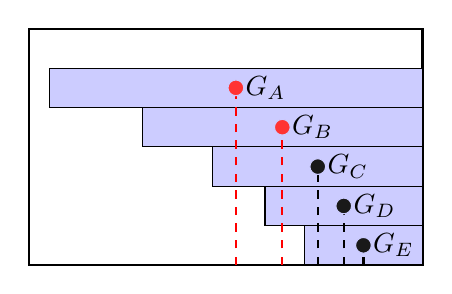
\begin{tikzpicture}
            % Draw the container
            \draw[thick] (0,0) rectangle (5,3);

            % Draw the three items inside
            % Draw the five items and their labels
            \draw[fill=blue!20] (3.5,0) rectangle (5,0.5);
            \draw[thick,dashed,black] (4.25,0) -- (4.25,0.25);  % <---
            \draw[fill = black!90, draw = blue!20] (4.25,0.25) circle (0.1);
            \node[anchor=west] at (4.25,0.25) {$G_E$};

            \draw[fill=blue!20] (3,0.5) rectangle (5,1);
            \draw[thick,dashed,black] (4,0) -- (4,0.75);  % <---
            \draw[fill = black!90, draw = blue!20] (4,0.75) circle (0.1);
            \node[anchor=west] at (4,0.75) {$G_D$};

            \draw[fill=blue!20] (2.33,1) rectangle (5,1.5);
            \draw[thick,dashed,black] (3.67,0) -- (3.67,1.25);  % <---
            \draw[fill = black!90, draw = blue!20] (3.67,1.25) circle (0.1);
            \node[anchor=west] at (3.67,1.25) {$G_C$};

            \draw[fill=blue!20] (1.44,1.5) rectangle (5,2);
            \draw[thick,dashed,red] (3.22,0) -- (3.22,1.75);  % <---
            \draw[fill=red!80, draw = blue!20] (3.22,1.75) circle (0.1);
            \node[anchor=west] at (3.22,1.75) {$G_B$};

            \draw[fill=blue!20] (0.26,2) rectangle (5,2.5);
            \draw[thick,dashed,red] (2.63,0) -- (2.63,2.25);  % <---
            \draw[fill=red!80, draw = blue!20] (2.63,2.25) circle (0.1);
            \node[anchor=west] at (2.63,2.25){$G_A$};


            %\node at (4, 1.875) {Fragile};
            %\node[anchor = west,align=center] at (2.9,2.5) {\small Center of \\  balance};

        \end{tikzpicture}
        \caption{Feasible, but unrobust, stacking with 75\% support area.}
    \end{subfigure}
    \hfill
    % Second TikZ picture
    \begin{subfigure}[b]{0.45\textwidth}
        \centering
        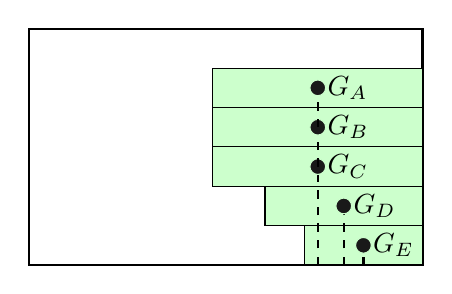
\begin{tikzpicture}
            % Draw the container
            \draw[thick] (0,0) rectangle (5,3);
            % Draw the three items inside
            % Draw the five items and their labels
            \draw[fill=green!20] (3.5,0) rectangle (5,0.5);
            \draw[thick,dashed,black] (4.25,0) -- (4.25,0.25);  % <---
            \draw[fill = black!90, draw = green!20] (4.25,0.25) circle (0.1);
            \node[anchor=west] at (4.25,0.25) {$G_E$};

            \draw[fill=green!20] (3,0.5) rectangle (5,1);
            \draw[thick,dashed,black] (4,0) -- (4,0.75);  % <---
            \draw[fill = black!90, draw = green!20] (4,0.75) circle (0.1);
            \node[anchor=west] at (4,0.75) {$G_D$};

            \draw[fill=green!20] (2.33,1) rectangle (5,1.5);
            \draw[thick,dashed,black] (3.67,0) -- (3.67,1.25);  % <---
            \draw[fill = black!90, draw = green!20] (3.67,1.25) circle (0.1);
            \node[anchor=west] at (3.67,1.25) {$G_C$};

            \draw[fill=green!20] (2.33,1.5) rectangle (5,2);
            \draw[thick,dashed,black] (3.67,1.25) -- (3.67,1.75);  % <---
            \draw[fill = black!90, draw = green!20] (3.67,1.75) circle (0.1);
            \node[anchor=west] at (3.67,1.75) {$G_B$};

            \draw[fill=green!20] (2.33,2) rectangle (5,2.5);
            \draw[thick,dashed,black] (3.67,1.75) -- (3.67,2.25);  % <---
            \draw[fill = black!90, draw = green!20] (3.67,2.25) circle (0.1);
            \node[anchor=west] at (3.67,2.25) {$G_A$};


            %\node at (4, 1.875) {Fragile};
            %\node[anchor = west,align=center] at (2.9,2.5) {\small Center of \\  balance};

        \end{tikzpicture}
        \caption{Feasible and robust stacking regarding 75\% support area.}
    \end{subfigure}
    \caption[Comparison of different vertical stability constraints.]{Comparison of different vertical stability constraints \\ with G = Center of Gravity (container side view). \footnotemark}
    \footnotetext{Own figures based on \textcite[p. 845]{krebs_advanced_2021}.}
    \label{fig:vertical_stability_comparison}
\end{figure}


\cite{gendreau_tabu_2006} showed, that the considered set of constraints for the \gls{CLP} significantly
changes the complexity and solution quality for the \gls{3L-CVRP}. On average, the solutions are $15.87\%$ more
cost-efficient and the computational time was significantly lower, when no additional constraints are considered.\footcite[cf.][p. 348]{gendreau_tabu_2006}
The loading constraints are therefore crucial for pre-determining the computation time as well as the complexity and the applicability
of the solutions, which is essential for improving realistic scenarios.
The following section highlights classical solution approaches of the \gls{CLP} in \gls{3L-CVRP} scenarios.


\section{Classical Solution Approaches}
\label{sec:classical_solution_approaches}
The \gls{CLP} is a $NP$-hard combinatorial problem. \footcite[cf.][p. 11]{bortfeldt_constraints_2013}
Consequently, heuristics and metaheuristics were the dominating tools
in the early stages of this research field.\footcite[cf.][]{pisinger_heuristics_2002} The variety of methods
and their solution quality developed in recent years. \footcite[cf.][p. 23]{iori_exact_2021}
When the \gls{CLP} is considered as subproblem of the \gls{VRP}, the focus shifts from finding optimal
packing solutions to guaranteeing feasibility for the loading of one cost-wise optimal route. Therefore,
speed and reliability are the main indicators for a good algorithm.
The variety of three-dimensional \gls{CLP} algorithms, especially for exact methods, is in comparison to two-dimensional limited, as
\textcite{zhao_comparative_2016} elaborated in their survey.\footcite[cf.][]{zhao_comparative_2016}
The following Figure~\ref{fig:solution_methods_overview} presents an overview of different algorithms,
where the \gls{CLP} was solved as subproblem.
It is divided in three categories: constructive heuristics, metaheuristics
and exact methods. Hybrid methods and improvement heuristics are not explicitly shown in the figure,
as the former combines components from multiple categories, while the latter is subsumed within
metaheuristics. It needs to be noted, that heuristics can fail to identify a feasible solution
in comparison to exact algorithms, but are computationally very lightweight approaches.
The depicted solution methods are described next.

\begin{figure}[htbp]
    \centering
    \resizebox{0.55\linewidth}{!}
    {
        \begin{tikzpicture}[grow cyclic, text width=2.7cm, align=flush center,
                level 1/.style={level distance=3.5cm,sibling angle=120},
                level 2/.style={level distance=3.5cm,sibling angle=50}
            ]

            \node {Solution Techniques \gls{CLP}}
            child { node {Metaheuristics}
                    child { node {Simulated Annealing}
                            child{node{One Stage Local Search Solver}}}
                    child { node {Tabu Search}}
                    child { node {Evolutionary Algorithm}}
                    child { node {Augmented extreme point-based heuristic}}
                }
            child { node {Exact \\ Methods}
                    child { node {Constraint Programming}}
                    child { node {Mixed-integer programming}}
                }
            child { node {Constructive Heuristics}
                    child { node {Layer/ Wall/ Tower Building}}
                    child { node {Corner Point Algorithms}
                            child{node{Minimize Waste Area}}}
                    child { node {Bottom-Left-Fill}
                            child{node{Deepest-Bottom-Left-Fill}}}
                    child { node {Maximum Touching Perimeter}
                            child{node{Maximum Touching Area}}}
                    child { node {Tree Search Algorithm}}
                }
            ;

        \end{tikzpicture}
    }
    \caption{Overview of solution methods for the container loading problem.}
    \label{fig:solution_methods_overview}
\end{figure}



\subsubsection{Constructive Heuristics}
For obtaining an initial feasible solution, two primary strategies are commonly
used depending on the heterogeneity of the items. In cases where the items are weakly homogeneous,
the problem dimensionality is reduced from 3D to 2D by constructing either
\textit{walls} or \textit{layers} of similarly sized items. These structures fill one
dimension of the container, typically either length and height or width and length, thereby
simplifying the remaining problem space. Moreover, when the layers or walls have approximately
equal dimensions, horizontal and vertical stability constraints are met.
Beyond these two dominant approaches, several adaptations exist to address item heterogeneity.
For example, \textcite{gehring_genetic_1997} propose the construction of item
\textit{towers}, in which boxes are stacked on top of other items so that the base of the box is covered completely
by the box below it. This effectively reduces the dimensions from 3D to a 2D floor space arrangement,
similar to the \gls{PLP}.\footcite[cf.][pp. 402--406]{gehring_genetic_1997}
In the integrated approach that combines the \gls{VRP} and the \gls{CLP} to solve the subproblem of the \gls{2L-CVRP}
or \gls{3L-CVRP}, the most common heuristics are variations of the \gls{BLF} and \gls{MTP} algorithms.
The \gls{BLF} heuristic determines the order in which each consecutive item is placed as close as possible to the
bottom-left corner of the vehicle. The
first priority is the distance to the container wall in the back and the second priority the distance
to the left container wall. This leads to a placing pattern of filling each row of the container floor
consecutively.
When the \gls{LIFO} constraint is considered, \cite{iori_exact_2007} utilized a \textit{contour} line
to identify the last possible placement of each item on the floor. The \gls{MTP} was introduced by
\cite{zachariadis_guided_2009} and inserts the next item regarding the perimeter of the item which is connected
to other items or additionally also to the container wall.\footcite[cf.][p. 732f]{zachariadis_guided_2009}
For the three-dimensional problem the heuristics were adapted to generate also appropriate solutions, when
stacking and multiple layers of items are considered. In \cite{gendreau_tabu_2006}, the \gls{BLF} was
adapted so that the bottom (first priority) could also represent already placed items. This leads
to a placing pattern where walls are constructed consecutively from the container back to the rear. The
\gls{MTP} was adapted from \cite{tarantilis_hybrid_2009} by considering the three-dimensional
surface of all items (\gls{MTA}). \footcite[cf.][pp. 258--260]{tarantilis_hybrid_2009}
In the work from \cite{tao_effective_2015} a corner point method
was introduced, which aims to minimize the waste area (unused loading capacities or blocked space) by
defining all possible corner points for each item, where the item could be placed in all possible
orientations.\footcite[cf.][pp. 130--132]{tao_effective_2015} The \gls{DBLF} algorithm
is an adaption of the \gls{BLF} algorithm and was initially integrated in the \gls{3L-CVRP} by \cite{wang_two_2010}
and further used by \cite{krebs_advanced_2021}.
The core adaption is, that the first priority for placing any item is as far as possible in the back of the cargo
leading to a more dense packing.\footcites(cf.)()[pp. 259--263]{wang_two_2010}[p. 8f]{krebs_axle_2021}
Additionally, \cite{bortfeldt_hybrid_2012} introduced a tree search algorithm as part of a hybrid method,
where packing decisions are systematically explored through backtracking to find feasible loadings for
given routes, making it a search-based heuristic rather than a purely constructive approach.\footcite[cf.][p. 2251f]{bortfeldt_hybrid_2012}
Even though constructive heuristics are quite simple, they are still widely used because of their simplicity and efficiency to obtain fast solutions.
\footcite[cf.][pp. 11--13]{tamke_branch-and-cut_2024}

\subsubsection{Metaheuristics}
Once an initial packing is found, metaheuristics can be applied to improve it.
This allows to accept infeasible packings during the constructive step,
as it is possible that a feasible modification can be found during the improvement phase.
Therefore, an encoded solution representation, such as a permutation of items, is required
to conduct changes of the current solution. \Glspl{GA} were
used to either improve the walls, towers or layers found by the constructive heuristics
or by improving the quality of the permutation of all items. \footcite[cf.][]{gehring_genetic_1997}
\Gls{TS} is a widely used approach for \gls{BPP} and \gls{CLP}. It is based on
the idea of iteratively improving a solution by exploring its neighborhood and simultaneously
storing certain moves or complete solutions in a tabu list to forbid back-cycling to
previous solutions, feasible or infeasible ones. \footcite[cf.][p. 344f]{gendreau_tabu_2006}
\Gls{SA} has rarely been used as a standalone metaheuristic in the context of \gls{CLP}, but is often
combined with other approaches to benefit the temperature dependent acceptance criterion of
solutions. At the beginning of the algorithm the probability
to accept worse solutions is higher as the cooling precedes, as \gls{SA} mimics the cooling curve from hot metal shifting from diversification to
intensification. This helps the algorithm to escape local optima
early in the search and gradually transition into a more focused phase. \cite{ceschia_local_2013} suggests
the usage of a one-stage \gls{LS} solver, which is directly improving the order of the items being
loaded on the vehicles instead of the customers. By combining a \gls{LNS} as
well as \gls{SA}, the solutions are allowed to be infeasible during the procedure and becoming repaired afterwards.
Hence, nine loading heuristics, based on \gls{BLF} and \gls{MTP}, were implemented as selectable options.
This was the first work to
solve the loading and routing completely integrated on item level. \footcite[cf.][pp. 1142--1145]{ceschia_local_2013}
\cite{tamke_branch-and-cut_2024} implemented an augmented extreme point-based metaheuristic
to speed-up the exact \gls{3L-CVRP} algorithm by avoiding the usage of the \gls{CP} solver, whenever the heuristic
found a feasibile solution. This metaheuristic is based on the extreme point heuristic from \cite{zhang_evolutionary_2015},
but adds several diversification and intensification elements as perturbation and \gls{LS} to find
feasible and qualitative loading solutions for their exact algorithm.\footcite[cf.][pp. 11--13]{tamke_branch-and-cut_2024}
In their work \cite{kucuk_constraint_2022} propose a hybrid approach for solving \gls{3L-CVRP} solving the
masterproblem \gls{VRP} optimally with an exact solver and using an \gls{EA}
to solve the \gls{CLP}. The approach is very similar to using a \gls{GA}, but \gls{EA}
has a better structural design flexibility.\footcite[cf.][pp. 5--8]{kucuk_constraint_2022}

\subsubsection{Exact Algorithms}
Retrieving optimal solutions for the \gls{CLP} is computationally challenging in comparison
to finding good solutions with heuristics. The main difficulty is to represent packing
patterns and the constraints introduced in Section~\ref{sec:clp_definition} in a mathematical way.
Two prominent methods exist for modeling the \gls{CLP}. The first one is \gls{LP}, which can be
formulated in two primary ways. The first approach defines each possible packing pattern as
a variable. \footcite[cf.][p. 29f]{zhu_prototype_2012} The second approach models
the placement of items using discrete coordinate variables. Each placement of an item
is defined by the cartesian coordinate tupel of the depeest, leftest and lowest corner point of
the item.\footcites(cf.)()[][pp. 649--653]{junqueira_optimization_2013}[][pp. 4--8]{moura_integrated_2009}
The second main method is \gls{CP}, which offers a flexible alternative for handling
complex constraints, where the focus is to find feasible solutions primarily and
not fulfilling an optimization criterion directly. \textcite{iori_exact_2021} states, that
\gls{CP} improved the results of two-dimensional \gls{CLP} problems significantly and is a promising
field of future research.\footcite[cf.][p. 23]{iori_exact_2021} \cite{tamke_branch-and-cut_2024} used a \gls{CP} solver
to solve the loading of single tours and were the first authors to introduce an exact algorithm
considering many loading constraints. \footcite[cf.][pp. 7--11]{tamke_branch-and-cut_2024}
A similar approach was conducted by \cite{hokama_branch-and-cut_2016}, which extended their
branch-and-cut approach, to be able to solve three-dimensional packings as well.
They also used a \gls{CP} model for \gls{CLP} feasibility checks, but considered less loading constraints.\footcite[cf.][]{hokama_branch-and-cut_2016}

\parbreak

In general, exact methods are not capable of solving packings with many items and practical relevance
in reasonable computation time. In their study to exactly solve the \gendreauDataSetText instances with all loading constraints,
\cite{tamke_branch-and-cut_2024} could solve instances up to 41 customers with an optimality
gap below $5 \%$. Their results can be used to understand the structure
of optimal solutions to provide lower bounds and guidance for the development of future
heuristics. Another feasible approach to improve
the performance of exact algorithms is the use of speed-ups. Depending on the complexity of
the considered loading constraints, the loading feasibiltiy check is the computational
bottleneck in finding the optimal overall solution for the \gls{3L-CVRP}. \textcite{tamke_branch-and-cut_2024} attempted
to enhance the solution process by adding stronger cuts and implementing a set partitioning heuristic to identify better routes
more efficiently. As a result, fewer routes and corresponding CLP feasibility checks needed to be evaluated. In addition,
they employed the aforementioned augmented extreme point-based metaheuristic to further accelerate the feasibility checking process.
At a total runtime of 8 hours, the slowdown effect was mainly caused by the feasibility checks, which accounted for at least 35\%
of the total runtime in 5 out of 19 instances.\footcite[cf.][p. 2]{tamke_branch-and-cut_2024}
Instead of using algorithmic speed-ups, some modern approaches in the loading and routing field tried
to instrumentalize pretrained \gls{ML} models for boosting the solving progress.
These promising models can substitute parts of the algorithm's computation time by predicting solution
feasibility or by quickly identifying good solutions. This reduces the computational effort
in iterative procedures. These approaches will be further discussed in the next section.

\section{Motivation for Feasibility Prediction}
\label{sec:motivation_feasibility_prediction}
This section explores how \gls{ML} algorithms can enhance \gls{3L-CVRP} solution strategies,
highlighting both benefits and limitations. Papers, which use predictive methods to accelerate the computation time
will be analyzed and promising implications are shown. It is important to note, that
several \gls{ML} approaches address the \textit{on-line} \gls{BPP}, where the optimal placement
of individual items, arriving sequentially, must be determined.\footcite[cf.][p. 1]{ali_-line_2022}
Since this work focuses on the \textit{off-line} \gls{BPP}, where a placement for all items is determined
simultaneously, on-line approaches are not further considered.

\subsubsection{Feasibility Classifier of the \cgls{2L-CVRP}}
As the number of customers is increasing, the number of routes is growing exponentially and the number of
possible loading combinations even more. As shown in the exact \gls{3L-CVRP} algorithm from \cite{tamke_branch-and-cut_2024},
the feasibility checks of the loading are the limiting computational factor in
exploring the exact branch-and-bound tree for the optimal solution. \footcite[cf.][p. 22]{tamke_branch-and-cut_2024}
Instead of using a complementary heuristic for boosting the feasibility checks,
\textcite{zhang_learning-based_2022} used a binary classifier to predict the feasibility of the
loading of single tours to reduce the overall computation time in their exact branch-and-price \gls{2L-CVRP}
algorithm. The classifier labeled each loading of a respective route in infeasible or feasible, which
reduced the frequency of calling the exact feasibility checker by $87.22\%$ and reduced the computational time by averagely $54.12\%$.
The exact \gls{SP} algorithm is then only used when single routes are labeled as infeasible to avoid
omitting feasible tours or before complete solutions are accepted as new \gls{LB} or \gls{UB} of the
algorithm procedure to avoid false positive labeled routes. To train the binary classifying model,
50.000 tours were obtained by running the underlying column generation
algorithm with only the exact feasibility checker and saving the labeled routes.
In their paper, the authors have chosen a \gls{FFNN} model, a special type of \gls{ANN} model,
from the PyTorch Library and compared it with a \gls{LR} model. In this comparison, the \gls{FFNN} model had
an accuracy of at most $94.1\%$ and the \gls{LR} model had a significantly smaller value.
The models were trained in many epochs using the mini-batch gradient descent algorithm. The prediction and training
of the loading of tours is based on 17 hand-crafted features, capturing geometric
and spatial characteristics of the packing problem. These include the ratio of the total item area
to the container floor area, as well as the mean, standard deviation, minimum, and maximum of
the following four indicators:
\begin{itemize}
    \item[1.] The ratio of item width to item height.
    \item[2.] The ratio of item width to the container width.
    \item[3.] The ratio of item height to the container height.
    \item[4.] The ratio of each item’s area to the total container area.
\end{itemize}

Even though the results are very positive, substantial simplifications regarding the loading were assumed: Stacking
of items is prohibited and only the area of the items is considerated, reducing the number of items significantly.
Additionally, practical loading constraints as \gls{LIFO} or horizontal stability
were not explicitly considered, reducing the problem complexity and therefore increasing the possibility to describe
the loading pattern with numerical features. \footcite[cf.][]{zhang_learning-based_2022}

\subsubsection{Pallet Size Classifier for the \gls{PLP}}
Another use case for \gls{ML} in packing problems is presented by \textcite{aylak_application_2021},
who focus on selecting the optimal pallet size in the context of the \gls{PLP}. Here, a number of fixed items
need to be placed on pallets with fixed weight, length and height dimensions, with the aim of optimizing the volume utilization,
subsequently generating stability and minimizing the number of pallets needed. Based on real-life data,
three candidate pallet sizes were considered and the best packing pattern must be found for each packing
configuration. Then, multiple packing heuristics were applied to
generate feasible packing patterns and identify the best-performing. These are used as labels for several
\gls{ML} models, which were trained to predict the optimal pallet size based on the box
dimensions \{x,y,z\} and the demand quantity. Compared to the purely heuristic approach, the classifier-based
determination achieved a volume utilization improvement of $6.7\%$ and significantly reduced computation time.
However, the study did not consider additional constraints such as weight limits, stacking rules, or stability.\footcite[cf.][pp. 12--14]{aylak_application_2021}

\subsubsection{Reinforcement Learning for the \gls{3L-CVRP}}
Another approach was chosen by \cite{schoepf_using_2024}, arguing that single heuristics are too domain- as well as use-case-specific.
Instead, they propose the usage of a \gls{RL} model for both the routing and loading. \gls{RL} belongs
to the unsupervised \gls{ML} models, where an agent selects one of several options at every stage, relying on random choices or
on past actions, reinterpreting the feedback. The goal of the agent is to independently learn
the patterns. This leads to the highest reward respective the lowest loss. Even though the authors could not beat
the best cost results from heuristics solving the gendreau benchmark, they had significantly lower computation times and
a linear instead of exponential increase in computational effort for bigger instances. This means a radical improvement
and could open a complete new approach in optimizing logistic problems and is hence the motivation to propose, that \gls{RL}
models will be able to solve \gls{3L-CVRP} problems of large instances better and easier than currently dominating
algorithms. \footcite[cf.][]{schoepf_using_2024}

\parbreak

These examples demonstrate, that \gls{ML} models can be successfully integrated into existing \gls{3L-CVRP}
algorithms to reduce computation time and overall complexity, provided the model is well trained.
However, training such a model can be often time-consuming, and the practicality of both training and
integration must be carefully evaluated on a case-by-case basis. The most promising approach to
accelerate the solving process of existing routing an loading algorithms, is the one from \cite{zhang_learning-based_2022},
pretraining a binary classifier boosting the loading feasibility check. However, in this approach,
the number of loading constraints was relatively small, allowing the classifier
to be trained with a limited set of features. When more complex constraints, such as
\gls{LIFO} unloading rules or item fragility, are introduced the construction of numerical features that accurately
represent these constraints becomes significantly more challenging. It needs to be investigated, if
the results of such a classifier assure practical relevance, since real-world
scenarios, such as loading large containers or trucks, inevitably involve
more constraints than scientific research has considered up to this point in time. \footcite[cf.][p. 1f]{bischoff_issues_1995}
Therefore, the development of a classifier is not only demanding, but also
requires careful consideration to ensure a favorable cost-benefit ratio. The next section widens the perspective
on \gls{3L-CVRP} algorithms presenting both \gls{CLP} and \gls{VRP} solution strategies and relevant work.

\section{Literature Overview}
\label{sec:literature_overview}
The reviewed literature is categorized into three main groups: metaheuristics, exact approaches and blended approaches of heuristics
and \gls{ML}.
Since the focus of this thesis is on route-loading feasibility, routing algorithms
are not discussed in further detail. Notably, papers reporting improvements on the \gendreauDataSetText instances, primarily
advanced the loading algorithms, whereas the \gls{CLP} constitutes the bottleneck of the problem. To refine the comparison,
different sets of loading constraints are summarized in Table~\ref{tab:constraint_sets}
and grouped according to the authors, who introduced them first.
Table~\ref{tab:literature overview} provides an overview of various approaches solving the integrated routing and loading
problems, where methods used to optimize the master problem, the \gls{VRP}, are introduced.
Most heuristics rely on \gls{LS} neighborhoods embedded within a metaheuristic, such as \gls{SA}, \gls{LNS},
or \gls{TS}.
Across the three categories, metaheuristic approaches generally consider the largest number of loading constraints. This results
from the more complex definitions required in exact or \gls{ML}-based methods, as well as their higher computational demands.
Moreover, when extending from the \gls{2L-CVRP} to the \gls{3L-CVRP}, additional constraints beyond sequence feasibility must
be addressed, since loading becomes more complex.
The following chapter builds on these insights and introduces all components for the training of a binary classifier
to establish the foundation for a promising new \gls{3L-CVRP} algorithm with integrated \gls{ML} techniques.

\begin{table}[ht]
    \footnotesize
    \centering
    \setlength{\tabcolsep}{3pt}         % tighten intercolumn space (default ~6pt)
    \renewcommand{\arraystretch}{1.2}   % a touch more row height
    \begin{tabular}{@{}
            P{0.25\textwidth} % Author
            P{0.15\textwidth} % Set Symbol
            P{0.50\textwidth} % Problem
            @{}}
        \toprule
        \textbf{Author}            & \textbf{Set Symbol} & \textbf{Constraints}                                                                   \\
        \midrule
        \cite{gendreau_tabu_2006}  & $\mathcal{G}$       & z-Rotation, Fragility, LIFO, Sequence, Support Area                                    \\
        \cite{ceschia_local_2013}  & $\mathcal{C}$       & z-Rotation, Load Bearing Strength, Reachability, MLIFO, Robust Stability               \\
        \cite{krebs_advanced_2021} & $\mathcal{K}$       & z-Rotation, Load Bearing Strength, Reachability, MLIFO, Robust Stability, Axle Weights \\
        \cite{iori_exact_2007}     & $\mathcal{I}$       & Sequence, \gls{LIFO}                                                                   \\
        \bottomrule
    \end{tabular}

    \caption{Various sets of loading constraints defined by different authors. }
    \label{tab:constraint_sets}
\end{table}


\begin{table}[ht]
    \scriptsize
    \centering
    \setlength{\tabcolsep}{3pt}         % tighten intercolumn space (default ~6pt)
    \renewcommand{\arraystretch}{1.3}   % a touch more row height

    \begin{tabular}{@{}
            P{0.05\textwidth} % Number
            P{0.08\textwidth} % Year
            P{0.15\textwidth} % Author
            P{0.10\textwidth} % Problem
            P{0.17\textwidth} % Routing Algorithm
            P{0.20\textwidth} % Loading Algorithm
            P{0.12\textwidth} % Constraints
            @{}}
        \toprule
        \textbf{No} & \textbf{Year}                          & \textbf{Author}                          & \textbf{Problem} & \textbf{Routing Algorithm}    & \textbf{Loading Algorithm}                & \textbf{Constraints}            \\
        \midrule

        \multicolumn{7}{c}{\textbf{Metaheuristics}}                                                                                                                                                                                      \\
        \midrule
        1           & \citeyear{gendreau_tabu_2006}          & \citeauthor{gendreau_tabu_2006}          & 3L-CVRP          & 4-Opt \gls{LS} with Tabu List & \gls{BLF}                                 & $\mathcal{G}$                   \\
        2           & \citeyear{gendreau_tabu_2008}          & \citeauthor{gendreau_tabu_2008}          & 2L-CVRP          & \gls{TS}                      & \gls{MTP}                                 & $\mathcal{I}$                   \\
        3           & \citeyear{tarantilis_hybrid_2009}      & \citeauthor{tarantilis_hybrid_2009}      & 3L-CVRP          & Guided \gls{TS}               & 6 different Heuristics (\gls{MTP}, \dots) & $\mathcal{G}$                   \\
        4           & \citeyear{zachariadis_guided_2009}     & \citeauthor{zachariadis_guided_2009}     & 2L-CVRP          & Guided \gls{TS}               & \gls{MTP}                  \& \gls{BLF}   & $\mathcal{I}$                   \\
        5           & \citeyear{wang_two_2010}               & \citeauthor{wang_two_2010}               & 3L-CVRP          & \gls{TS}                      & \gls{DBLF} \& \gls{MTP}                   & $\mathcal{G}$                   \\
        6           & \citeyear{bortfeldt_hybrid_2012}       & \citeauthor{bortfeldt_hybrid_2012}       & 3L-CVRP          & \gls{TS}                      & Tree search algorithm                     &                                 \\
        7           & \citeyear{ceschia_local_2013}          & \citeauthor{ceschia_local_2013}          & 3L-CVRP          & \gls{SA} with \gls{LNS}       & Different Heuristics (\gls{BLF}, \dots)   & $\mathcal{C}$                   \\
        8           & \citeyear{tao_effective_2015}          & \citeauthor{tao_effective_2015}          & 3L-CVRP          & \gls{TS}                      & Least Waste Heuristic                     & $\mathcal{G}$                   \\
        9           & \citeyear{zhang_evolutionary_2015}     & \citeauthor{zhang_evolutionary_2015}     & 3L-CVRP          & Evolutionary \gls{LS}         & \gls{LS} with Open Space Heuristic        & $\mathcal{G}$                   \\
        10          & \citeyear{krebs_axle_2021}             & \citeauthor{krebs_axle_2021}             & 3L-CVRP          & Adaptive \gls{LNS}            & \gls{DBLF}                                & $\mathcal{G}$ + Axle Weights    \\
        11          & \citeyear{krebs_advanced_2021}         & \citeauthor{krebs_advanced_2021}         & 3L-CVRP          & Adaptive \gls{LNS}            & \gls{DBLF}                                & $\mathcal{K}$                   \\
        \addlinespace[0.5em]
        \midrule
        \multicolumn{7}{c}{\textbf{Exact Approaches}}                                                                                                                                                                                    \\
        \midrule
        12          & \citeyear{iori_exact_2007}             & \citeauthor{iori_exact_2007}             & 2L-CVRP          & Branch-and-cut                & Branch-and-bound \& \gls{BLF} Heuristic   & $\mathcal{I}$                   \\
        13          & \citeyear{junqueira_optimization_2013} & \citeauthor{junqueira_optimization_2013} & 3L-CVRP          & Integer \gls{LP}              & Branch-and-bound \& \gls{BLF} Heuristic   & Multidrop, \gls{LBS}, Fragility \\
        14          & \citeyear{hokama_branch-and-cut_2016}  & \citeauthor{hokama_branch-and-cut_2016}  & 2L/3L-CVRP       & Branch-and-cut                & \gls{CP} Solver \& Heuristic              & $\mathcal{I}$                   \\
        15          & \citeyear{tamke_branch-and-cut_2024}   & \citeauthor{tamke_branch-and-cut_2024}   & 3L-CVRP          & Branch-and-cut                & \gls{CP} Solver \& Heuristic              & $\mathcal{G}$                   \\
        \addlinespace[0.5em]
        \midrule
        \multicolumn{7}{c}{\textbf{Blended Approaches}}                                                                                                                                                                                  \\
        \midrule
        16          & \citeyear{kucuk_constraint_2022}       & \citeauthor{kucuk_constraint_2022}       & 3L-VRPTW         & CP-Solver                     & \gls{EA}                                  & Full rotation                   \\
        17          & \citeyear{zhang_learning-based_2022}   & \citeauthor{zhang_learning-based_2022}   & 2L-VRPTW         & Branch-and-price              & Binary Classifier + \gls{SP} Algorithm    & $\emptyset$                     \\
        18          & \citeyear{schoepf_using_2024}          & \citeauthor{schoepf_using_2024}          & 3L-CVRP          & \gls{RL}                      & \gls{RL}                                  & $\mathcal{G}$                   \\


        \bottomrule
    \end{tabular}

    \caption{Literature overview on different solution methods of the VRP
        with loading constraints.}
    \label{tab:literature overview}
\end{table}
